\section{Curva de rotación}

\subsection{Marco teórico}

Sea $P$ un punto a través de la línea de visión a longitud $l$ y distancia galactocéntrica $R=R_\odot\sin l$. Se supone $P$ bajo un movimiento puramente circular con velocidad $v_\textnormal{rot}(R)$, denominada velocidad rotacional, cuya componente a lo largo de la línea de visión con respecto al LSR, es decir, su velocidad radial medible a través del efecto Doppler, es $v_\textnormal{LSR}$, formando un ángulo $\alpha$ entre ambas, por lo tanto, contrarrestando la velocidad del Sol $v_\odot$ relativa a la línea de visión,
\begin{equation}
v_\textnormal{LSR}(R)=v_\textnormal{rot}(R)\cos\alpha-v_\odot\sin l
.\label{eq:vll}\end{equation}
Sea $\beta$ el ángulo interior que forma el Sol, el punto $P$ y el centro galáctico. Se aprecia que $\beta=90+\alpha$, y, usando el teorema del seno,
\begin{equation}
\frac{\sin l}{R}\equiv\frac{\sin\beta}{R_\odot}=\frac{\cos\alpha}{R_\odot}
,\end{equation}
de modo que la ecuación \ref{eq:vll} se reescribe como,
\begin{equation}
v_\textnormal{LSR}(R)=v_\textnormal{rot}(R)\frac{R_\odot\sin l}{R}-v_\odot\sin l
,\label{eq:nomaestra}
\end{equation}
y, definiendo la velocidad angular mediante la siguiente relación,
\begin{equation}
v_\textnormal{rot}(R)=\omega(R)R
,\end{equation}
se obtiene la ecuación maestra de la cinemática de la Galaxia,
\begin{equation}
v_\textnormal{LSR}(R)=\left(\omega(R)-\omega(R_\odot)\right)R_\odot\sin l
.\label{eq:maestra}\end{equation}

Para una misma velocidad $v_\textnormal{LSR}(R)$, existe una doble ambigüedad en la distancia heliocéntrica $D$ del punto $P$ que le corresponde, pues, dentro del círculo solar, la línea de visión intersecta a la circunferencia de radio $R$ en un punto cercano y en otro lejano. Esto no ocurre fuera del círculo solar.

Es importante determinar la distancia $D$ para poder calcular la densidad numérica y densidad de masa gracias a la luminosidad, y, si no se determina, solo se puede calcular la densidad de columna.

Sea $D_\textnormal{N}$ la distancia cercana y $D_\textnormal{F}$ la distancia lejana. Geométricamente, se obtiene,
\begin{equation}
D_{\substack{F\\N}}=R_\odot\cos l\pm\sqrt{R^2-R_\odot^2\sin^2l}
\end{equation}

La velocidad máxima $v_\textnormal{LSR}^{\max}(R)$ que se puede medir en la línea de visión ocurre en el punto $P$ sobre esta que tiene la menor distancia galactocéntrica $R_{\min}=R_\odot\sin l$, suponiendo $\omega$ monotónicamente decreciente con respecto a $R$, lo que se puede establecer con el modelo de distribución de masa de disco de la Galaxia, que se estudia en la sección \ref{sec:massmodel} y sugiere $\omega\propto R^{-1/2}$. Este punto se denomina punto subcentral. Su distancia heliocéntrica es $D_\textnormal{N}=D_\textnormal{F}=R_\odot\cos l=D_{\tan}$, su velocidad tangencial o rotacional es, gracias a la ecuación \ref{eq:nomaestra}.
\begin{equation}
v_\textnormal{rot}(R_\odot\sin l)=v_\textnormal{LSR}(R_\odot\sin l)+v_\odot\sin l
,\label{eq:vrot}\end{equation}
y su velocidad angular es,
\begin{equation}
\omega(R_\odot\sin l)=\frac{v_\textnormal{LSR}}{R_\odot\sin l}+\omega(R_\odot)
.\label{eq:wrot}\end{equation}

Las velocidades rotacionales permitidas en la galaxia interna, en donde $R<R_\odot$ y luego $\omega(R)>\omega(R_\odot)$, para el cuarto cuadrante galáctico, en donde las longitudes está en el rango $\ang{270}<l<\ang{360}$, de modo que $\sin l<0$, cumplen, según la ecuación \ref{eq:maestra}, con $v_\textnormal{LSR}(R)<0$, es decir, efecto Doppler con corrimiento al azul.

\subsection{Detalle del algoritmo}

La curva de rotación se deriva de las velocidades terminales del espectro de CO para cada longitud galáctica $l$. El cuarto cuadrante galáctico tiene emisión con corrimiento al azul, por lo tanto, se escogen las velocidades terminales más negativas posibles para cada espectro y que cumplan cierta condición que se explica a continuación. El procedimiento corresponde al código \ref{cod:vrot} y se hacen los cálculos utilizando valores absolutos cuando corresponda, para tener bien definidos los radios y velocidades rotacionales como positivos, puesto que en este cuadrante el seno de la longitud es negativo.

Se utiliza la técnica de \textit{sigma clipping} para obtener la base de ruido de los espectros con un número de tres y media desviaciones estándar para el límite de recorte tanto superior como inferior, además de las iteraciones necesarias para que el algoritmo converja. Suponiendo que el promedio del ruido se anula, entonces la temperatura de ruido o valor RMS del ruido es igual a la desviación estándar del mismo.

La velocidad terminal se define para cada longitud $l$ y para cada latitud $b$ como aquella velocidad del primer punto del espectro de emisión cuya temperatura sea cinco veces mayor a la temperatura de ruido, considerando primero las velocidades del lado del corrimiento al azul del espectro, es decir, recorriendo el espectro desde la velocidad más negativa a la más positiva. Esta condición se muestra en la figura \ref{fig:vterminal}.

A continuación, se escoge para cada longitud $l$ el máximo maximorum entre las velocidades terminales de todas las latitudes $b$.

\begin{figure}[htbp]
	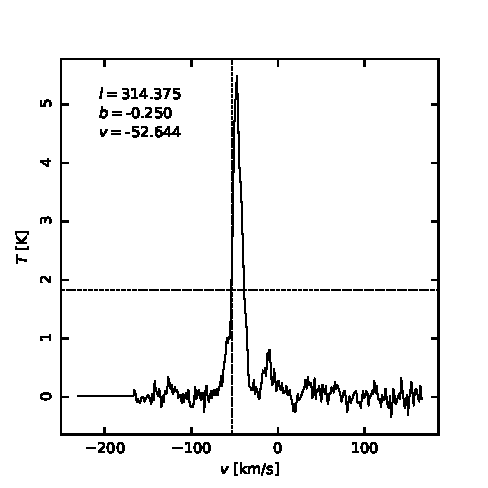
\includegraphics{rsc/vterminal.pdf}
	\caption{Un típico espectro de emisión, para las coordenadas $l=\ang{314.385}$ y $b=\ang{-0.250}$, con la condición para elegir la velocidad terminal. La línea discontinua horizontal representa un nivel de $5\sigma$ de ruido. La primera temperatura del lado del corrimiento al azul en superar esta condición ocurre a una velocidad $v_\textnormal{LSR}=\SI{-52.644}{\kilo\metre\per\second}$, que corresponde a la línea discontinua vertical.}
	\label{fig:vterminal}
\end{figure}

\subsection{Curva de rotación: $v_{\textnormal{rot}}$ vs. $R$ y \mbox{$\omega$ vs. $R$}}

Se usa la ecuación \ref{eq:vrot} y los máximos maximorum de velocidades terminales para graficar en la figura \ref{fig:vrot} las velocidades rotacionales para cada longitud.

Se utiliza la ecuación \ref{eq:wrot} junto con los máximos maximorum de velocidades terminales para graficar en la figura \ref{fig:w} las velocidades angulares para cada longitud.

\begin{figure}[htbp]
	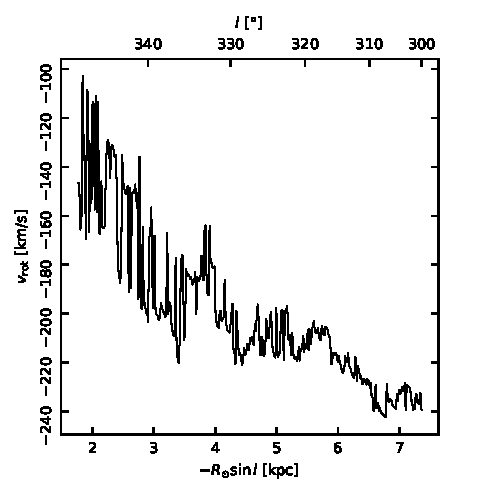
\includegraphics{rsc/vrot.pdf}
	\caption{Curva de rotación del cuarto cuadrante galáctico. Velocidad rotacional, correspondiente al máximo maximorum de velocidades terminales de las latitudes, en función de la distancia galactocéntrica (eje inferior) y la longitud (eje superior).}
	\label{fig:vrot}
\end{figure}

\begin{figure}[htbp]
	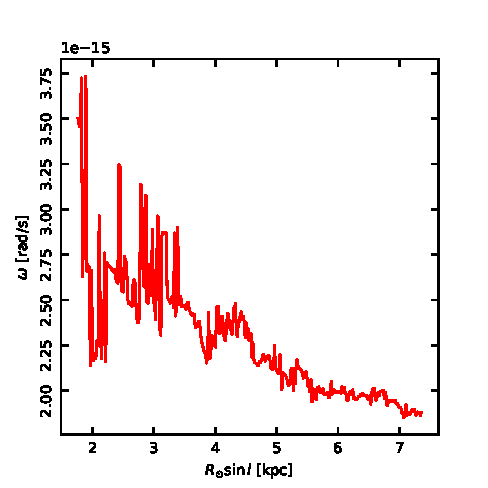
\includegraphics{rsc/w.pdf}
	\caption{Curva de rotación del cuarto cuadrante galáctico. Velocidad angular de cada máximo maximorum de velocidad terminal en función de la distancia galactocéntrica (eje inferior) y la longitud (eje superior).}
	\label{fig:w}
\end{figure}
